\subsection{Metrics for Performance Evaluation}
\label{sec:neural-networks-metrics}
When the training of a network is finished, its performance needs to be expressed in numbers.
There are several common metrics available, that depend on some definitions that will be introduced first.
A true positive $TP$ is a correct prediction of a sample, so the positive class is predicted correctly.
A true negative $TN$ is a correct rejection of a sample, i.e. the network knows that a certain sample does not belong to a certain category.
Hence, it predicts correctly the negative class.
Furthermore, a false positive $FP$ is a wrong prediction of a sample.
The network incorrectly predicts the positive class.
The last definition is a false negative $FN$.
This means the network incorrectly predicts the negative class.
Their connection is visualized in \figref{fig:confusion-matrix} showing the so-called confusion matrix \cite{Fawcett:2006:IRA:1159473.1159475} for the example class Class A.
In this case, Class B represents Not Class A.
\begin{figure}
	\centering
	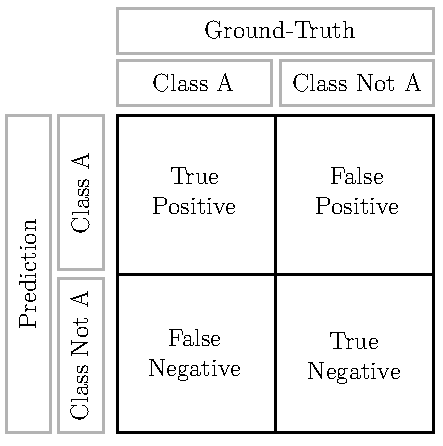
\includegraphics[]{images/confusion_matrix.pdf}
	\caption[Confusion matrix]{Confusion matrix for class A, where Class B represents Not Class A.}
	\label{fig:confusion-matrix}
\end{figure}
One metric is the accuracy
\begin{equation}
	ACC = \frac{TP + TN}{TP + TN + FP + FN}
\end{equation}
of the model.
This states how many samples the network correctly classifies.
However, this metric's results are not reliable for the real performance, because it highly depends on the dataset.
If it is unbalanced like if there are more samples in a well classifiable category than in a bad one, the accuracy is shifted.
The precision or positive predicted value of a network measures how accurate the predictions are and is calculated by
\begin{equation}
	\label{eq:metric-precision}
	PPV = \frac{TP}{TP + FP}
\end{equation}
where the denominator refers to the total positive results.
Furthermore, the recall or true positive rate metric measures how good all positives are found by
\begin{equation}
	\label{eq:metric-recall}
	TPR = \frac{TP}{TP + FN}
\end{equation}
where the denominator refers to the actual positives.